\chapter{JUDUL BAB...}
Contoh gambar..
\begin{figure}[H]
\centering
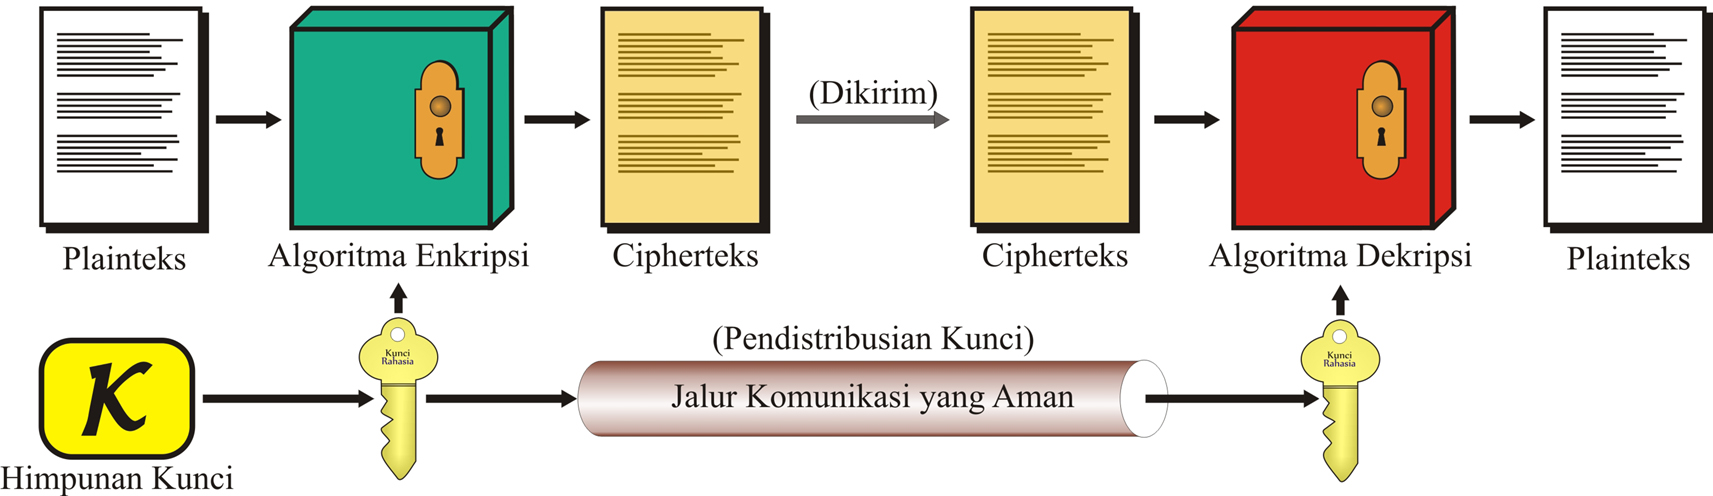
\includegraphics[width=12cm]{skemasimetris}
\caption{Diagram ilustrasi}
\end{figure}
\bigskip
\begin{figure}[H]
\centering
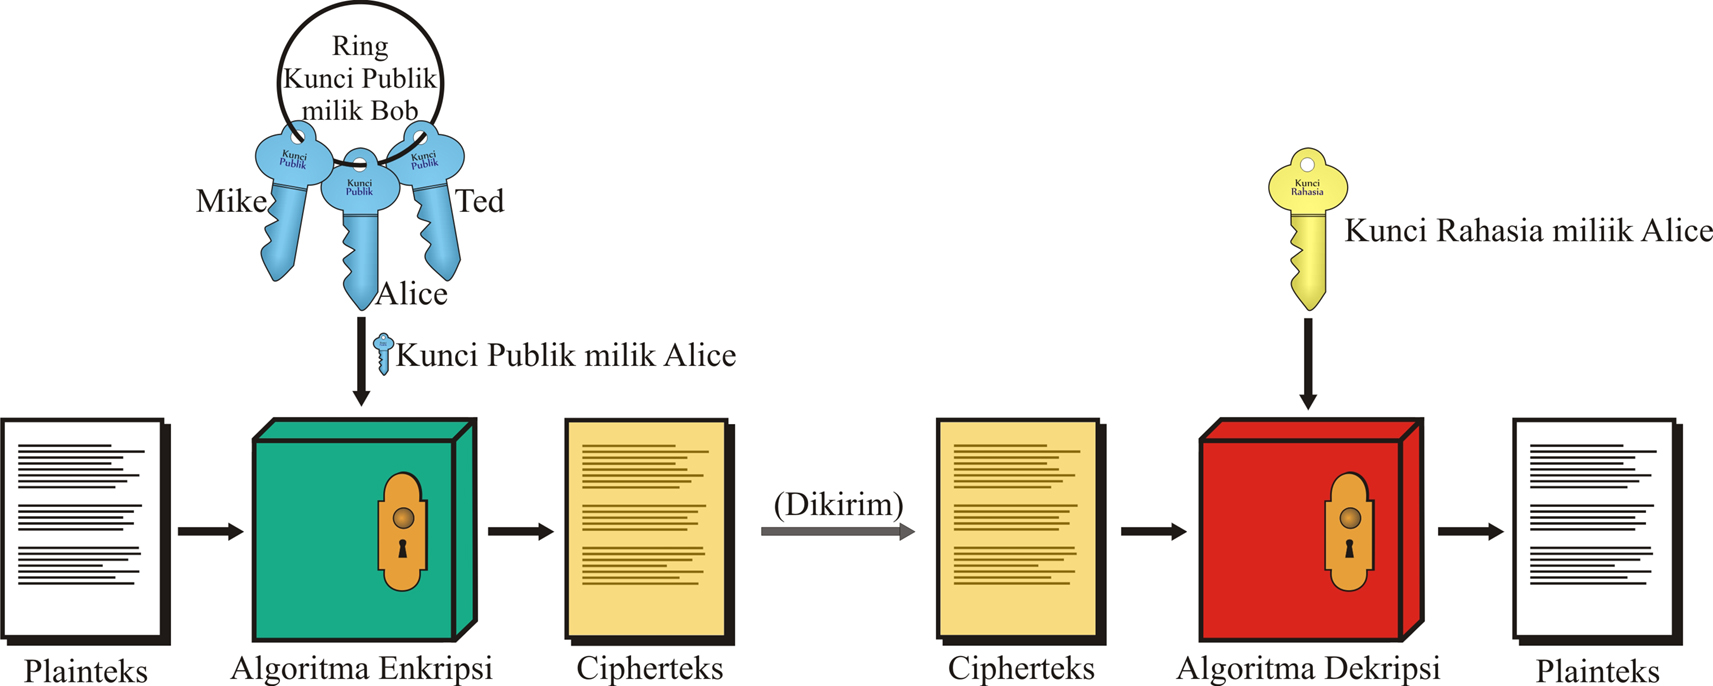
\includegraphics[width=12cm]{skemaasimetris}
\caption{Diagram ilustrasi}
\end{figure}

Contoh tabel...
\begin{longtable}{|c|c|c|c|c|}
 \caption{Hasil Panen Padi}\label{tran7}\\
 \hline
  Kota Jogja&Bantul&Sleman&Kulon Progo&Gunung Kidul \\
  \hline
  55 & 164 & 91 & 239 & 921 \\
  \hline
  13 & 70 & 187 & 295 & 629 \\
  \hline
  3 & 96 & 37 & 525 & 645 \\
  \hline
  6 & 221 & 61 & 175 & 666 \\
  \hline
  64 & 84 & 4 & 133 & 571 \\
  \hline
  50 & 5 & 20 & 259 & 257 \\
  \hline
  33 & 3 & 396 & 749 & 461 \\
  \hline
  10 & 6 & 41 & 43 & 535 \\
  \hline
  33 & 22 & 108 & 370 & 840 \\
  \hline
  & 77& 398 & 321 & 857 \\
  \hline
  & 250 & 172 & 474 & 402 \\
  \hline
  & 167 & 111 & 327 & 57 \\
  \hline
  & 17 & 328 & 225 & 299 \\
  \hline
  & 30 & 7 & 346 & 644 \\
  \hline
  &  & 28 & 455 & 1.984 \\
  \hline
  &  & 224 & 143 &  \\
  \hline
  &  & 63 & 256 &  \\
  \hline
  &  & 146 & 190 &  \\
  \hline
  &  & 69 & 436 &  \\
  \hline
  &  & 254 & 62 &  \\
  \hline
  &  & 192 & 528 &  \\
  \hline
\end{longtable}


\begin{longtable}{|ccccccc|}
\caption{Penduduk dan Pertumbuhannya }\label{tran3}\\
\hline
 \multicolumn{3}{|c}{Penduduk Bantul} & & \multicolumn{3}{c|}{Penduduk Sleman} \\
  \hline
   Tahun  &   Penduduk    &   Pertumbuhan   &    &  Tahun    &  Penduduk     & Pertumbuhan\\
  \hline
  1990 & 1,86  &      &    & 1990 & 22,16  &  \\
  1992 & 2,34  & 0,48 &    & 1992 & 29,13  & 6,97 \\
  1994 & 2,78  & 0,44 &    & 1994 & 37,21  & 8,08\\
  1996 & 3,21  & 0,43 &    & 1996 & 48,28  & 11,07 \\
  1998 & 4,22  & 1,01 &    & 1998 & 60,12  & 11,84\\
  2000 & 6,21  & 1,99 &    & 2000 & 74,51  & 14,39\\\hline
\end{longtable}